\chapter{How to Have the Best Year Ever}

This chapter follows Jim Rohn's seminar talk ``How to Have the Best Year Ever,'' preserved not as a clean institutional course but as part of a curated playlist assembled by LazyingArt LLC. The original speaker is Jim Rohn, and the formal content is therefore not blackboard mathematics in the usual sense; it is a practical calculus of self-management, built from ratios, repeated acts, and causal chains. Because no validated mathematical frames survive for this lecture, every diagram below is a transcript-derived schematic reconstruction. We shall keep close to the lecture's actual motion: first the contract of the day, then the story that authorizes the teaching, then the five-part life model, and finally the applied domains of goals, money, communication, and resolve.

\section{Investment, Story, and Seminar Terms}

Rohn opens with comedy and then almost immediately closes the trap. The day is not entertainment. It is an investment. One may recover money; one does not recover time. That is the first inequality of the lecture, and it governs everything that follows:
\begin{equation}
T > M,
\end{equation}
where \(T\) denotes time and \(M\) denotes money. The point is not algebraic elegance. It is evaluative force. If a seminar merely returns its fee, it has done the lesser part of its job; if it returns a day, it has justified itself at the higher level.

This opening contract also explains the speaker's self-presentation. He does not ask us to admire a polished performer. He asks us to judge whether the day yields value. The autobiography that follows is therefore not ornament. It is evidence. We move from Idaho farm country, to quitting college too early, to marriage and mounting embarrassment, to creditors, broken promises, and the painful recognition that hard work without a governing philosophy can still produce pennies in the pocket and nothing in the bank.

The decisive event is the arrival of Earl Shoaff. Rohn's narrative authority rests here. He meets a man who is both wealthy and teachable as an example. Shoaff teaches books, disciplines, language, personality, and method. In Rohn's own telling, this does not merely improve a circumstance. It changes income, bank balance, future, and life-direction. The autobiographical sequence serves one exact purpose: before he gives us formulas, he shows us a case in which those formulas operated.

A second transition follows. Having been coached, Rohn later discovers that his story itself has market value. He is asked to speak, then paid to speak, and then builds a speaking and writing life out of translated experience. That is important for the rest of the chapter. The lecture will repeatedly insist that ideas become powerful only when translated into disciplined action and then into communicable value.

\section{How to Listen}

The lecture next defines its own method. We are not asked merely to agree, still less merely to applaud. We are asked to be sincere, alert, thankful, and studious. The first distinction is crucial:
\begin{equation}
\mathrm{Sincerity} \neq \mathrm{Truth}.
\end{equation}
Rohn's point is sharp. A speaker may be sincere and still be wrong. Sincerity proves only sincerity. Truth must be tested by truth. In a seminar of this kind, that is a vital epistemic warning, because strong personality and strong feeling can otherwise masquerade as proof.

\subsection{Question \& Answer}

\paragraph{Question.} If sincerity is not truth, how is truth tested?

\paragraph{Answer.} By the lecture's own rule, sincerity tests sincerity and nothing more. Truth must be checked against what is true, against results, against reality, against the numbers, and against the disciplined consequences of acting on an idea. The correct response to a sincere speaker is therefore not passive obedience but active study. We are to be students, not followers.

That stance immediately illuminates the next pair, ideas and inspiration. Rohn does not oppose them; he joins them. We need ideas because life can change by means of one more idea in a chain already partly assembled. His model is the lock combination:
\begin{equation}
(n_1,\dots,n_k,n_{k+1}) \Rightarrow \text{lock opens}.
\end{equation}
The point is that one more number may suffice when several are already in place. The seminar, a sermon, a conversation, a song lyric, or a scene from a film may supply precisely that missing term. This is not mysticism. It is a combinatorial image for delayed breakthrough.

At the same time inspiration remains mysterious. Some people come, some do not. Some change, some do not. Rohn refuses to over-systematize this. He accepts a crude but durable empirical law: in every field there are those who do and those who do not. The lecture therefore advises us not to waste our attention trying to ``de-perplex the perplexed.'' It asks instead for gratitude, listening, and good notes.

Two practical rules conclude the section. First, be thankful: gratitude opens channels that cynicism closes. Second, do not become a disciple. ``Take advice, but not orders.'' The action worth taking must become the product of one's own conclusion. That is already one of the lecture's hidden mathematical habits: external input must be processed into an internally owned rule before it becomes durable.

\section{The Five Pieces of the Life Puzzle}

Rohn now introduces the main scaffold of the lecture. The five major pieces are philosophy, attitude, activity, results, and lifestyle. In the lecture's order, and also in its logic, they run as
\begin{equation}
P \to H \to A \to R \to L,
\end{equation}
where \(P\) is philosophy, \(H\) attitude, \(A\) activity, \(R\) results, and \(L\) lifestyle.

This sequence is not presented as an airtight theorem. It is a practical causal order. Philosophy comes first because it governs how we interpret everything else. Rohn's characteristic metaphor is that philosophy is ``the set of the sail.'' The winds may be shared, but the sail-setting is personal. One person blames the economy, the schools, the taxes, the company, or the weather; another trims the sail.

Because no validated lecture frames survive, the following diagram is a transcript-derived schematic reconstruction rather than a recovered board figure.

\begin{figure}
\begin{center}
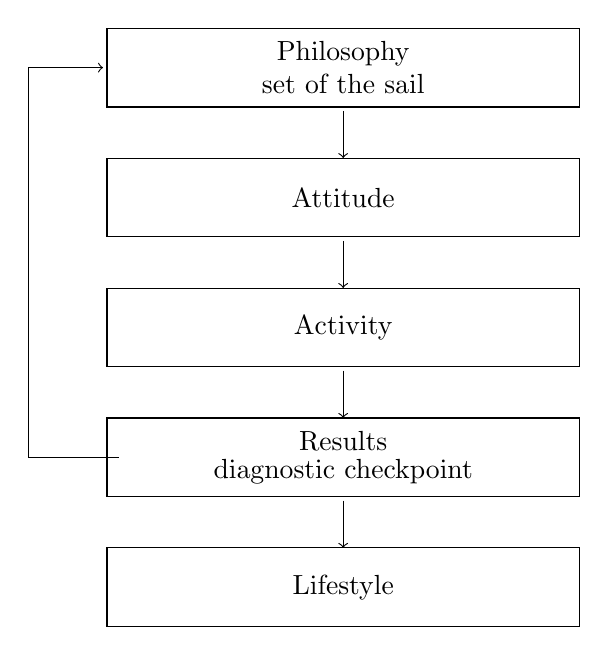
\begin{tikzpicture}[x=1cm,y=1cm]
\draw (0,0) rectangle (6,1);
\node at (3,0.5) {\shortstack{Philosophy\\set of the sail}};

\draw[->] (3,-0.05) -- (3,-0.65);

\draw (0,-1.65) rectangle (6,-0.65);
\node at (3,-1.15) {Attitude};

\draw[->] (3,-1.70) -- (3,-2.30);

\draw (0,-3.30) rectangle (6,-2.30);
\node at (3,-2.80) {Activity};

\draw[->] (3,-3.35) -- (3,-3.95);

\draw (0,-4.95) rectangle (6,-3.95);
\node at (3,-4.45) {\shortstack{Results\\diagnostic checkpoint}};

\draw[->] (3,-5.00) -- (3,-5.60);

\draw (0,-6.60) rectangle (6,-5.60);
\node at (3,-6.10) {Lifestyle};

\draw[->] (0.15,-4.45) -- (-1.0,-4.45) -- (-1.0,0.50) -- (-0.05,0.50);
\end{tikzpicture}
\end{center}
\end{figure}

The feedback arrow matters. The lecture does not say this in formal notation, but it clearly implies it:
\begin{equation}
R \to P_{\text{revised}}.
\end{equation}
Results do not terminate the sequence. They diagnose it. If the results are poor, then philosophy must be revisited; if the results are strong, philosophy has acquired confirmation.

Rohn's strongest argument for the primacy of philosophy is built from what cannot be changed. We arrive in a world already stocked with seed, soil, rain, sunshine, seasons, markets, schools, and institutions. In his rhetoric these are the givens. If we blame them wholesale, we are blaming all we have to work with. The lecture's practical metaphysics is therefore austere: the materials are given; the handling of them is not.

\subsection{Question \& Answer}

\paragraph{Question.} If the seasons and circumstances do not change, what exactly can we change?

\paragraph{Answer.} We change the inner ordering principle. We change philosophy, and from that point attitude, activity, results, and lifestyle may begin to change as well. This is why the lecture insists, again and again, that the real work is not to request another planet or another economy, but to alter the way the present world is read and used.

The second piece, attitude, is briefly defined by its stable parts: attitude toward the past, toward the future, toward other people, and toward oneself. Even where the transcript later becomes noisy, this structure survives intact. But attitude is still not first. The lecture expressly says that life change does not begin with inspiration or mood. It begins with education. That is to say: first see correctly, then feel correctly.

\section{Errors, Disciplines, and Results}

Once the five-piece scaffold is erected, the lecture tightens into formulas. These are the nearest thing this seminar has to equations of motion:
\begin{align}
\mathrm{Failure} &= \text{a few errors in judgment, repeated every day},\\
\mathrm{Success} &= \text{a few simple disciplines, practiced every day}.
\end{align}
The speaker's method here is excellent. He does not leave these formulas in the air. He drives them into a small bodily example: the apple and the Hershey bar. ``An apple a day'' is not interesting because it is nutritionally sophisticated. It is interesting because it is small, easy, repeatable, and therefore cumulative. A Hershey bar in place of the apple is not a catastrophe in one evening. It is a catastrophe in seed form.

The lecture's point is not that disaster arrives instantly. It is rather that delayed consequences deceive the undisciplined. The first day without the apple does not end in sickness. The first day without the walk around the block does not end in collapse. This delay is precisely what makes neglect dangerous. The process hides its own trajectory.

The lecture therefore gives a paired practical formula:
\begin{equation}
\mathrm{could}+\mathrm{should}+\mathrm{don't/won't}\Rightarrow \mathrm{disaster},
\end{equation}
while the reversal produces the opposite motion:
\begin{equation}
\mathrm{could}+\mathrm{should}+\mathrm{will}\Rightarrow \mathrm{change}.
\end{equation}

\subsection{Question \& Answer}

\paragraph{Question.} If the right act is so simple, why is change still rare?

\paragraph{Answer.} Because, in Rohn's language, what is easy to do is also easy not to do. Simplicity does not remove resistance; it exposes it. Small neglect is dangerous not because it is large, but because it repeats without immediate penalty. Small discipline is powerful for the same reason. Both accumulate.

Results now enter as the lecture's auditing device. Philosophy, attitude, and activity must submit to number. Rohn's teacher does not ask for stories. He asks how much money has been saved and invested, how many books have been read, how many classes have been taken, how many calls have been made, how many pounds have been gained. This is why the lecture can summarize the whole topic so abruptly: ``Results is the name of the game.''

One may compress that audit schematically as
\begin{equation}
R=(n_{\text{books}},\, n_{\text{classes}},\, n_{\text{calls}},\, \Delta w,\, s,\dots),
\end{equation}
with the warning that the lecture itself is verbal and practical rather than formally statistical. The meaning is plain: results come in countable forms.

\paragraph{Worked example.} Rohn's own sales illustration is simple enough to serve as a model. If a salesperson is supposed to make ten calls in a week, then
\begin{align}
n_{\text{calls}}^{\text{target}} &= 10,\\
n_{\text{calls}}^{\text{actual}} &= 1 \quad \text{or} \quad 20.
\end{align}
The lecture's point is that the number already reveals a philosophy, an attitude, and an activity-pattern. A story is secondary. The number does the diagnostic work.

This is why the lecture says that life asks only for measurable progress in reasonable time. It is also why it insists that success is a numbers game. Numbers do not replace moral judgment here; they prevent excuses from replacing judgment.

\section{Personal Development and the Seasonal Cycle}

The next large movement broadens the frame. We now move from isolated disciplines to personal development as a whole. Rohn's formula is familiar and severe: if we wish to have more, we must become more. The external world does not need to rearrange itself first. We do not wait for circumstances to soften. We work on ourselves harder than we work on the job. That is the lecture's great transfer of effort from environment to person.

The largest metaphor in this middle movement is seasonal:
\begin{equation}
(\mathcal W,\mathcal{Sp},\mathcal{Su},\mathcal F)
=
(\text{winter},\text{spring},\text{summer},\text{fall}).
\end{equation}
Rohn's definitions are practical rather than meteorological:
\begin{align}
\mathcal W &= \text{adversity to be handled},\\
\mathcal{Sp} &= \text{opportunity to be seized},\\
\mathcal{Su} &= \text{a time to nourish and protect},\\
\mathcal F &= \text{harvest to be reaped without complaint}.
\end{align}

The following diagram is again a transcript-derived schematic reconstruction.

\begin{figure}
\begin{center}
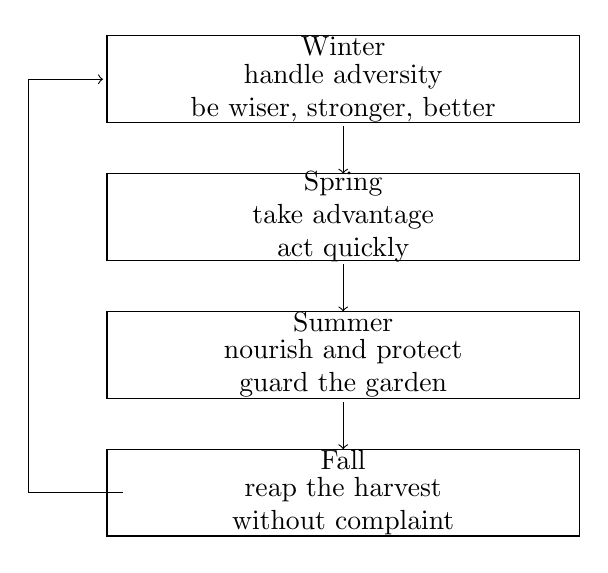
\begin{tikzpicture}[x=1cm,y=1cm]
\draw (0,0) rectangle (6,1.1);
\node at (3,0.55) {\shortstack{Winter\\handle adversity\\be wiser, stronger, better}};

\draw[->] (3,-0.05) -- (3,-0.65);

\draw (0,-1.75) rectangle (6,-0.65);
\node at (3,-1.20) {\shortstack{Spring\\take advantage\\act quickly}};

\draw[->] (3,-1.80) -- (3,-2.40);

\draw (0,-3.50) rectangle (6,-2.40);
\node at (3,-2.95) {\shortstack{Summer\\nourish and protect\\guard the garden}};

\draw[->] (3,-3.55) -- (3,-4.15);

\draw (0,-5.25) rectangle (6,-4.15);
\node at (3,-4.70) {\shortstack{Fall\\reap the harvest\\without complaint}};

\draw[->] (0.2,-4.70) -- (-1.0,-4.70) -- (-1.0,0.55) -- (-0.05,0.55);
\end{tikzpicture}
\end{center}
\end{figure}

The logic is memorable. We do not pray away winter; we learn how to handle it. We do not merely enjoy spring; we take advantage of it. We do not merely enjoy summer growth; we defend it against weeds, insects, and threats. We do not blame the harvest; we reap what comes and take responsibility.

This seasonal model lets Rohn bring together several strands that would otherwise seem separate. The library belongs here because getting wiser is one way of preparing for winter. The journal belongs here because reflecting on days, weeks, months, and years is one way of gathering the past and investing it into the future. The five abilities belong here as well:
\begin{enumerate}
\item absorb,
\item respond,
\item reflect,
\item act,
\item share.
\end{enumerate}
The sequence is exact. First one takes in the day. Then one lets the day touch feeling. Then one reflects on it, so that experience is not wasted. Then one acts before intent decays. Finally one shares, which enlarges capacity and prepares the person to hold more of the next experience.

The lecture's ``law of diminishing intent'' belongs here. The moment of clear idea and strong emotion is unstable. If it is not translated into action, it cools. That is why Rohn repeatedly urges immediate small discipline: get the book now, write the letter now, start the push-ups now, begin the library now. The emphasis is not theatrical urgency; it is respect for how fast intention evaporates.

\section{Goals and Designed Future}

We come now to the second great pivot of the lecture. Shoaff asks a devastating question: where is the list of goals? Rohn has no list. Shoaff replies that he can guess the bank balance of a man who has no list of goals. This is one of the lecture's deepest transitions: vagueness about the future is not neutral. It already has measurable economic consequences.

Goals are defined as one's vision of the future. More exactly, they distinguish two ways of facing the future:
\begin{equation}
F_{\text{undesigned}} \Rightarrow \mathrm{apprehension},
\qquad
F_{\text{designed}} \Rightarrow \mathrm{anticipation}.
\end{equation}
The undesigned future produces hesitant steps. The designed future produces active movement. Hence the lecture's sharp counsel: if one does not make one's own plans, one will fall into someone else's plans, and someone else's plans may amount to ``not much.''

Rohn attaches a second formula to this transition:
\begin{equation}
\text{price is easy if the promise is clear}.
\end{equation}
That is psychologically exact within the terms of the lecture. People do not ordinarily refuse discipline because discipline is impossible. They refuse it because the promise is dim. When the future becomes visible, the price becomes bearable. Thus the lecture's advice is practical and almost embarrassingly simple: decide what you want and write it down.

\subsection{Question \& Answer}

\paragraph{Question.} Why set a millionaire goal if money itself is not the deepest value?

\paragraph{Answer.} Because the major value of the goal lies in what it makes of the person who pursues it. This is Shoaff's famous correction, and it changes the meaning of ambition at once. The goal is large not because the cash is sacred, but because the stretch required to reach it reorganizes the person.

The lecture makes this explicit:
\begin{equation}
\text{greatest value in life} \neq \text{what you get},
\qquad
\text{greatest value in life} = \text{what you become}.
\end{equation}
We are therefore asked to ask a higher question at work, in enterprise, and in pursuit: not merely ``What am I getting?'' but ``What am I becoming?''

This deeper account of goals is immediately balanced by warning. Do not set goals too low. Do not join an easy crowd. Go where expectations are high, where pressure to grow is real, and where one cannot remain the same. But also do not sell out. Count the cost. The lecture's Judas example, however rhetorically charged, is used for one rigorous point: a gain purchased at the price of self-betrayal is not a gain. One must mark well what one becomes in pursuit of what one wants.

\section{Financial Independence, Communication, and Resolve}

\subsection{Financial Independence as Applied Philosophy}

The lecture now turns from goal-setting to explicit money rules. The key transition is that economics is used as a visible part of personal development because it is countable. We are not paid for time as such; we are paid for value brought to the marketplace. Hence another sharp distinction:
\begin{equation}
\text{pay} \neq \text{time}.
\end{equation}
Time is the container. Value is the priced content. Therefore, if \(V\) denotes value brought to the marketplace and \(Y\) the resulting income, the practical rule becomes
\begin{equation}
V \mapsto 2V \Rightarrow Y \mapsto 2Y,
\end{equation}
with the lecture's own qualification that this increase may occur ``in the same time.'' That is the value ladder. One does not get rich by demand alone. One becomes more valuable.

Rohn's sample personal-finance rule is equally direct:
\begin{align}
S &\le 0.70I,\\
C &= 0.10I,\\
K_a &= 0.10I,\\
K_p &= 0.10I,
\end{align}
where \(I\) is income, \(S\) spending, \(C\) charity, \(K_a\) active capital, and \(K_p\) passive capital. The corresponding warning is
\begin{equation}
O>I \Rightarrow \text{downfall},
\end{equation}
with \(O\) for outgo.

\paragraph{Worked example.} If one takes the lecture's own pedagogical unit of one dollar and scales it to \(I=100\), then the plan reads
\begin{align}
I &= 100,\\
S &\le 70,\\
C &= 10,\qquad K_a=10,\qquad K_p=10.
\end{align}
If instead one lives at \(O=110\), then the deficit is immediate:
\begin{equation}
O-I = 10.
\end{equation}
Rohn's point is not to produce household-finance theory. It is to show that even a crude plan beats no plan, and that ``it is not the amount that counts; it is the plan that counts.''

He then distinguishes the three main channels in simple language:
\begin{itemize}
\item wages help make a living;
\item profits help make a fortune;
\item interest is what passive capital earns when someone else uses the money.
\end{itemize}
Accordingly,
\begin{equation}
\text{profits}>\text{wages}
\end{equation}
in the narrow sense relevant here: profits have greater wealth-building power. The same holds for lending:
\begin{equation}
\text{borrower} \prec \text{lender}.
\end{equation}
The power position is not the spender but the lender.

The finance block contains one more important correction of attitude. Taxes, in Rohn's formulation, are how one feeds ``the goose that lays the golden eggs.'' Bills, likewise, can be reframed as liability reduction and asset improvement. We need not accept every rhetorical flourish here to see the mechanism: attitude toward obligation changes conduct, and conduct changes result.

\subsection{Communication}

The lecture's communication theory is more structured than it first appears. It is built from four stages. First, have something good to say. Second, say it well. Third, read the audience. Fourth, use intensity without excess. The preparatory side matters most. Words can work miracles only if they carry substance.

Rohn's strongest metaphor here is that words can create light. That claim is theological in origin, but its practical use is plain: a speaker may bring another person from darkness into visibility. In a more compact practical form, the lecture's communication law is
\begin{equation}
\text{well-chosen words}+\text{measured emotion}\Rightarrow \text{strong communication}.
\end{equation}
The adjective ``measured'' is essential. Emotion without measure becomes overkill. Hence the lecture's maxim: do not shoot a cannon at a rabbit.

The second strong claim is that vocabulary is a way of seeing. A limited vocabulary narrows both perception and expression. The argument is not merely literary; it is behavioral. If one cannot see finely and cannot express finely, judgment deteriorates. Hence the emphasis on reading, on a ``word for the day,'' and on the systematic expansion of language.

To read an audience, the lecture recommends three channels:
\begin{itemize}
\item read what you see;
\item read what you hear;
\item read what you feel.
\end{itemize}
That triad is enough for the chapter. The more corrupted stretches of the transcript add examples, but the structure itself is stable and clear.

\subsection{Resolve and the Final Turn}

The closing movement joins negative and positive motivation. Negative is not to be ignored; it is to be mastered. The ant thinks winter in summer. One must not be fooled by blue skies into building on sand. That is the lecture's way of insisting that difficulty is normal, not anomalous.

The positive turn then comes in four stages:
\begin{equation}
\text{disgust} \to \text{decision} \to \text{desire} \to \text{resolve}.
\end{equation}
Disgust is the moment of ``I've had it.'' Decision cleans up the list. Desire is triggered and intensified by experience. Resolve says ``I will.'' The lecture's preferred final word is not promise in the abstract but perseverance in the concrete: until. Read until understanding changes. Practice until skill changes. Walk until strength changes. Keep going until the new pattern is established.

This closing machinery is immediately turned outward. Help people with their lives, not just their jobs. Help them with books, poems, words, goals, dreams, errors, and futures. The last reliable sentence of the lecture gives the chapter its final line of force: if one works on one's gifts, those gifts make room.

\section{Summary}

The lecture begins by ranking time above money and ends by claiming that developed gifts create room for a life. Between those two claims it builds a practical chain. First comes philosophy, then attitude, then activity, then results, and finally lifestyle. Failure and success are both cumulative. Goals convert apprehension into anticipation. Economic independence depends less on amount than on plan, less on hours than on value. Communication turns inner development outward. Resolve sustains the whole structure until it bears fruit.

What makes the chapter distinctive is that none of these claims are offered as detached abstractions. Each is introduced through story, resistance, and example: the Idaho farm boy, the apple and the Hershey bar, the ten calls, the library card, the goal list, the dollar split, the widened vocabulary, the seasons, and the final insistence that one help people with their lives. The lecture's formal content is therefore schematic but not thin. It is a lived mathematics of repetition, proportion, accumulation, and feedback, ordered by one governing conviction: if we change, everything changes.